\chapter
 [Architecture of an Operating System for a Quantum Network Node]
 {Architecture of an\\Operating System for a\\Quantum Network Node}
\label{chp:arch}

\begin{abstract}
The end goal of an \acrfull{os} for quantum network nodes is to bridge the gap between user
applications --- written in high-level and platform-independent software --- and the underlying
quantum hardware, to which the user is agnostic. How can one design a control system that adheres to
this objective, while addressing the challenges that come with quantum networking? And what does an
example architecture of such a system look like? This chapter explores the cardinal design
considerations that should drive the design of an \acrshort{os} for quantum network nodes, and
proposes a proof-of-principle architecture for such an \acrshort{os}.
\end{abstract}

\blfootnote{
    This chapter is extracted from the article in preparation:
    \fullcite{delledonne_2023_qnodeos_noprint}.
}

\newpage

\lettrine{A}{n} \acrfull{os} is usually the cornerstone of a system's control software: it manages
and marshals access to physical resources, abstracts low-level hardware functionalities into
user-friendly services, and provides an interface to users to program and run applications on the
system. Our goal here is to apply basic principles from classical \acrshort{os} design literature to
our novel use case of programmable and scalable quantum networking nodes, and to (hopefully) create
a framework where the challenges outlined in \cref{chp:background} can be studied and addressed. We
thus investigate the general requirements that such a system should satisfy, illustrated with the
example of a quantum processor based on \acrfull{nv} centers in diamond. This provides a guideline
for future systems of this form. We also propose the \emph{first proof-of-principle architecture for
an \acrlong{os} for quantum network nodes}, which we call \acrshort{qnodeos}. Our system's
capabilities include quantum memory management, scheduling different types of quantum operations on
the device, as well as an interface to different drivers addressing several possible quantum
hardware architectures. On the quantum networking front, \acrshort{qnodeos} adopts the quantum
network stack and protocols proposed by \textcite{dahlberg_2019_egp} and by
\textcite{kozlowski_2020_qnp}.

\section{General Design Considerations}
\label{sec:arch:considerations}

We assume that the operating system builds upon a quantum hardware system capable of the execution
of \emph{physical instructions} addressing specific qubits on the quantum chip. These physical
instructions may be dependent on the type of quantum hardware (e.g. \acrshort{nv} in diamond, or ion
traps), and include instructions for initializing and measuring qubits on the chip, moving the state
of a qubit to another location in the quantum memory, performing quantum gates, as well as to make
attempts at entanglement generation at the physical layer~\cite{pompili_2022_experimental}. The
quantum hardware furthermore exposes the capabilities of the quantum chip: (1) the number of qubits
(2) the type of each qubit (3) the memory lifetime of the qubits (4) the physical instructions that
can be performed on on the qubit(s) and (5) the average quality of these instructions
(\cref{chp:background}). We emphasize that, unlike in classical computing, there is currently no
established low-level microarchitecture that defines the line between (quantum) hardware and
software upon which such an operating system would be built. We nevertheless expect that almost all
of the below would be functions taken on by any operating system, some of which could possibly be
shifted to control hardware in the future.

Each node in the network runs its own independent quantum network operating system. Nodes may
interact with each other using both classical message passing as well as entanglement generation.
The goal of the combined system is to execute quantum network applications, which themselves consist
of separate programs running on the operating system(s) of two (or more) network nodes. Such
programs generally also communicate via classical message passing and entanglement generation. Each
program itself consists of both classical and quantum blocks of code, where the quantum blocks of
code may contain low-level classical logic (specifically, branching on classical variables and
loops). Classical blocks of code may depend on quantum ones via classical variables generated during
the quantum execution (measurement results, notification of entanglement generation, and information
on the state of the quantum system such as the availability of qubits). Similarly, quantum blocks
may depend on variables set by the classical blocks, such as messages received from remote network
nodes. Finally, quantum blocks may themselves depend on other quantum blocks via qubits in the
quantum memory. It is the responsibility of the programmer or compiler to identify what is a
classical and what is a quantum block. Similarly, we assume that (potentially fine-grained)
deadlines or priorities in the execution are determined by the programmer (or compiler) using the
knowledge of the exposed capabilities of the quantum hardware system (e.g. memory lifetimes).
Determining precise deadlines (e.g. when too much time has elapsed for the qubits to be useful) is
in general a computationally expensive procedure, sometimes estimated in practice by a repeated
simulation of the execution. We remark that there is no way in quantum mechanics to measure the
current quality of a qubit or operation during the ongoing execution, and such qualities are
determined by performing estimates independently of the program execution itself. Of course, the
operating system could itself engage in such estimates when idling in order to update its knowledge
of the capabilities of the quantum hardware.

\section{Key OS Components}
\label{sec:arch:components}

We now describe the essential components we envision any operating system for quantum network nodes
to have.

\subsection{Memory Management Unit}

Executing quantum network applications demands a continuing interaction between the classical and
quantum parts of the execution, including keeping qubits alive in memory to take further actions
depending on messages from remote network nodes. We thus require persistent memory management
capabilities. This may be taken up by a \emph{\acrlong{qmmu}} (\acrshort{qmmu}). A \acrshort{qmmu}
has knowledge of the physical qubits available on the underlying quantum hardware, and may keep any
other information about said qubits, such as the qubit type (communication or storage qubit) and
qubit lifetime. A \acrshort{qmmu} allows physical qubits to be assigned to different applications or
to the operating system itself, and may allow a transfer of ownership of the qubits from one owner
to another. A \acrshort{qmmu} may also provide abstractions familiar to classical computing such as
a virtual address space, where the applications refer to virtual qubit addresses that are then
translated to physical qubit addresses. This avoids the situation in which physical qubit addresses
must be bound at compile time, particularly limiting when allowing multiple applications to
concurrently run on the same node. Advanced forms of a \acrshort{qmmu} may also cater to the
limitations of near term quantum devices, by matching memory lifetime requirements specified by the
application code to the capabilities of the underlying qubits, as well their topology (i.e. taking
into account which two qubits allow two-qubit gates to be performed on them directly). While one
cannot measure the decoherence of a qubit during a general program execution on the quantum level,
the \acrshort{qmmu} could also take into account additional information from the classical control
system to signal to the application that a qubit has become invalid.

\subsection{Quantum Network Stack}

The \acrshort{os} should include the capability for quantum communication with remote nodes in the
network, typically the generation of entanglement. We thus assume that the \acrshort{os} realizes a
quantum network stack that can be relied upon to enable entanglement generation, where we refer to
Ref.~\cite{dahlberg_2019_egp} for design considerations of quantum network stacks themselves. The
network stack allows an application to request a certain number or rate of entangled pairs to be
produced with remote nodes with a specified quality (i.e. fidelity) of entanglement. The stack is
responsible for ensuring the delivery of the entanglement. One possible quantum network stack can be
found in Ref.~\cite{dahlberg_2019_egp} including the first link layer protocol now realized on
quantum hardware~\cite{pompili_2022_experimental} (as described in \cref{chp:netstack}), and a
network layer protocol (as proposed in Ref.~\cite{kozlowski_2020_qnp}).

To successfully produce entanglement, the network stack needs access to a communication qubit,
resulting in two requirements for the rest of the system:

\begin{enumerate}
    \item A scheduler should take into account that generating entanglement at the physical layer
          between two nodes directly connected by a physical communication medium requires that the
          two nodes apply a series of physical operations with very precise timing synchronization
          between them (nanosecond precision with sub-nanosecond jitter). Therefore, entanglement
          generation across a link with an adjacent node must always be scheduled in a synchronized
          manner between the two adjacent neighbors. Similarly, due to limited memory lifetimes,
          generating entanglement with the help of an intermediary node at the network
          layer~\cite{kozlowski_2020_qnp} requires specific operations (entanglement swapping) to be
          scheduled at all three nodes within a time window allowed by the memory lifetimes.
    \item On some quantum hardware systems (e.g. \acrshort{nv} in diamond), the communication qubit
          is in general needed to enable the execution of quantum gates on and in-between storage
          qubits. This has implications both on the scheduler (local instructions cannot be
          scheduled concurrently to networked ones), as well as on the \acrshort{qmmu}, which needs
          to allow qubit ownership transfer between applications and the network stack. A typical
          use case of such ownership transfer would occur when the network stack claims the
          communication qubit for entanglement generation, and then yields it to an application.
\end{enumerate}

\subsection{Scheduler}

In order to maximize the usage of resources, we envision the \acrshort{os} to include a scheduler.
This may be a single scheduler, or more likely several schedulers that address scheduling at
different levels. In general, we may consider scheduling at the level of applications, at the level
of blocks of quantum code, and at the level of instructions, each level not being independent of one
another.

\paragraph{General considerations}

A scheduler for quantum network nodes should be capable of managing the limited physical resources
to achieve the desired performance. The performance of any form of scheduling method in the quantum
domain is assessed not only by existing classical metrics --- like throughput and latency --- but
also by quantum metrics (see \cref{chp:background}). At the level of the application, latency can be
measured in terms of the success probability of the quantum network application. At the level of an
operation (or a block of operations) it may be measured by the quality (fidelity) of the quantum
states and operations performed. We remind that due to limited memory lifetimes, delays have always
a direct impact on the quantum performance, resulting in general in trade-offs between classical and
quantum performance metrics when assessing any scheduler.

Practically, the scheduler in question should allocate the underlying physical resources --- most
importantly, the qubits --- based on a set of well-defined constraints, the fundamental ones being:

\begin{enumerate}
    \item \emph{Synchronized network schedule}: due to the bilateral nature of entanglement, each
          node will have its quantum networking activity synchronized with its neighbors, meaning
          that a missed synchronization window on one node results in a waste of resources on remote
          nodes too.
    \item \emph{Local quantum computation}: in addition to quantum networking, a node's resources
          must also be reserved for local quantum gates, which are integral parts of quantum
          networking applications.
    \item \emph{Inter-block dependencies}: quantum and classical processing blocks of an application
          may depend on results originating from other blocks, and thus cannot be scheduled
          independently.
    \item \emph{Multitasking}: for a node to be shared by multiple users, the scheduler should not
          allocate all the available resources to a single application indefinitely, and instead it
          should be aware of the presence of multiple applications and multiple users.
\end{enumerate}

Additionally, scheduling at any level could optionally process another set of input variables, where
we generally assume that the programmer or compiler provide aggregate advice based on these input
variables to the \acrshort{os}:

\begin{enumerate}
    \item \emph{Duration of operations}: local quantum operations typically take a fixed amount of
          time and always succeed. Entanglement, on the other hand, is a probabilistic process, and
          generating an entangled pair can take an indefinite (and large) number of attempts.
          Scheduling decisions may factor this in to yield better performance.
    \item \emph{Decoherence}: as already stated, the fidelity of a quantum state stored in a qubit
          is not constant, and it also degrades due to physical noise induced by other qubits and by
          operations applied on such qubits. An advanced scheduler could use knowledge of qubit
          lifetimes and elapsed time to dynamically re-prioritize application demands based on the
          advice of the compiler.
\end{enumerate}

\paragraph{Scheduling of applications}

In an \acrshort{os} allowing the execution of concurrent quantum network applications, the task of
an application-level scheduler would be to decide which application to schedule next. We remark that
a programmer (or compiler) aware of the underlying capabilities of the hardware system (e.g. memory
lifetimes) can provide advice in the form of a deadline by which the network application must have
completed in order to be successful. To allow for potentially time-consuming classical pre- and
post-processing, it is natural to apply such deadlines not for the entirety of the application, but
for the period between initializing the qubits and terminating the quantum part of the execution.
This suggests in general using real-time schedulers for quantum network applications, taking
inspiration from the extensive work on this topic in classical systems (see e.g.
Ref.~\cite{liu_1973_scheduling}). While outside the scope of this work, we remark that this type of
scheduling offers to inspire interesting new work in a form of ``quantum soft-real time''
scheduling, where deadlines may occasionally be missed at the expense of reduced application
performance (success probability), to maximize the overall performance of the system in which
applications are typically executed repeatedly. A benchmark for the quantum performance of any
application-level scheduler is the quality of the quantum execution when the entire system (all
nodes) are reserved for only one application at the time.

\paragraph{Scheduling of quantum blocks}

Scheduling can also (additionally) be performed on the level of quantum blocks of code. This can in
principle also take the form of a (soft) real-time scheduler that schedules blocks of the currently
running application, or schedule blocks of several applications (potentially independently of any
application level scheduling) depending on the availability of resources on the quantum hardware
system. This form of scheduling may be appealing for efficiency reasons, depending on where what
parts of the operating system are executed, where some parts are closer to the underlying hardware
system than others (see e.g. \cref{sec:arch:design}).

\paragraph{Scheduling of operations}

Finally, scheduling can be performed at two levels of operations: First, one can consider the
problem of scheduling local versus networked instructions, where one simple way of realizing a
schedule that respects the constraints inherent in such a schedule is presented in
\cref{sec:arch:design}. Second, one can consider scheduling any form of operation on the underlying
quantum processor. While our current realization of \acrshort{qnodeos} achieves this by populating
an instruction queue in software, we envision that this form of scheduling would later be moved from
\acrshort{qnodeos} to a hardware module in a microarchitecture for quantum networking nodes, as for
instance in the work by \textcite{fu_2017_microarch}.

\section{QNodeOS Design}
\label{sec:arch:design}

\acrshort{qnodeos} is an operating system for quantum network nodes, designed to address the
challenges described in \cref{chp:background}. It includes all the identified key components, plus
some additional convenience abstraction layers. The current design of \acrshort{qnodeos} is
considered \emph{best-effort} --- it is meant to explore the main design aspects of an operating
system for quantum networks, and to provide a minimum working system.

\subsection{Full Stack of a Quantum Network Node}

As described in \cref{chp:background} and illustrated in \cref{fig:app-struct}, a quantum network
application consists of programs running on different end nodes, composed of blocks of quantum code
and blocks of fully-classical code. In fact, quantum code blocks may also contain simple classical
logic --- like simple arithmetic and branching instructions --- used for flow control. These blocks
do not have any dependencies on data originating from other nodes. Fully-classical code blocks ---
which include local processing and communication with other end nodes --- mainly produce input data
for the next quantum code blocks. That is, a classical code block typically precedes a quantum code
block whose instructions depend on external data coming from a remote end node. In our system,
quantum code blocks expressed in \emph{NetQASM}~\cite{dahlberg_2022_netqasm}. NetQASM is an
open-source \acrfull{sdk} and instruction set for quantum applications~\cite{netqasm_sdk}. The
NetQASM \acrshort{sdk} compiles a quantum network application, written in Python, into a series of
classical and quantum code blocks. The instruction set used for the quantum code blocks is similar
to other QASM languages~\cite{cross_2017_qasm, khammassi_2018_cqasm, fu_2019_eqasm}, but it is
extended to include instructions for quantum networking. NetQASM is not a strict requirement of
\acrshort{qnodeos}, but it does impose certain conventions (described in
Ref.~\cite{dahlberg_2022_netqasm}) on a particular implementation of the system.

In principle, classical and quantum code blocks can be run on a single system, provided that this
has a connection to the quantum device to execute the actual quantum instructions. However, in the
interest of a simpler implementation, where each system has a scoped responsibility, we opted to map
classical and quantum blocks onto two distinct environments. Classical blocks are run on a system
that features a fully-fledged \acrshort{os} (like Linux), with access to high level programming
languages (like C++ and Python) and libraries. Quantum blocks are delegated to the
\emph{\acrlong{qnpu}} (\acrshort{qnpu}), which is a system capable of interpreting quantum code
blocks and managing the resources of a quantum device. In our design, a quantum network application
starts on the general-purpose \acrshort{os} --- that we call the \emph{host} --- which runs
classical code blocks internally, and offloads quantum code blocks to the \acrshort{qnpu}.
\acrshort{qnodeos} is the topmost component of the \acrshort{qnpu}. It runs the quantum code blocks,
relying on the underlying quantum device --- denoted as \emph{\acrshort{qdevice}} --- to execute the
actual quantum operations.

The architecture of a quantum network node is depicted in \cref{fig:quantum-node}. An alternative
architecture could merge host and \acrshort{qnodeos} into the same system, potentially enabling some
performance optimizations, at the cost of a higher system complexity. We also note that the host,
\acrshort{qnodeos} and the classical control modules of the \acrshort{qdevice} can be deployed on
distinct physical devices, or combined in some way.

\begin{figure}[t]
    \centering
    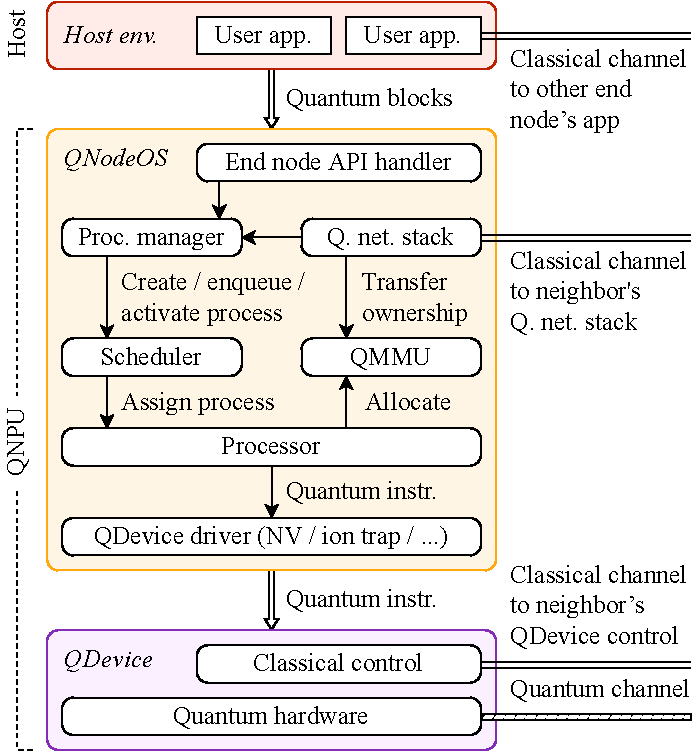
\includegraphics[width=0.6\linewidth]{figures/quantum-node.pdf}
    \caption{
        Full-stack architecture of a quantum network node. User applications start in the host
        environment, which runs classical code blocks and offloads quantum code blocks to the
        \acrshort{qnpu}. \acrshort{qnodeos}, lying at the top of the \acrshort{qnpu}, processes
        quantum code blocks and invokes the quantum device (\acrshort{qdevice}) to run the actual
        quantum instructions. \acrshort{qnodeos} consists of an end-node \acrshort{api} handler, a
        quantum network stack (Q. net. stack), a process manager (Proc. manager), a quantum memory
        management unit (\acrshort{qmmu}), a scheduler, a processor, and a \acrshort{qdevice} driver
        to communicate with the \acrshort{qdevice} itself. The host shares a classical communication
        channel with other end nodes' hosts for application data. \acrshort{qnodeos} shares a
        classical channel with its neighbors. The \acrshort{qdevice} shares a classical channel for
        coordination and a quantum channel for entanglement with its neighbors.
    }
    \label{fig:quantum-node}
\end{figure}

\subsection{Processes}

A quantum network application starts on the host --- there, the host environment compiles it into
classical and quantum code blocks, and creates a new process associated with the application. The
host then registers the application with \acrshort{qnodeos} (through \acrshort{qnodeos}'s end-node
\acrshort{api}), which, in turn, creates its own process associated with the registered application.
The process on the host is a standard \acrshort{os} process, which executes the classical code
blocks and interacts with the counterpart process on \acrshort{qnodeos} (by means of a shared
memory, as defined in NetQASM~\cite{dahlberg_2022_netqasm}). On \acrshort{qnodeos}, a process
encapsulates the execution of quantum code blocks of an application with associated context
information, such as process owner, ID, process state and priority.

The execution time of an application is typically dominated by that of quantum blocks, as
entanglement generation is a time-consuming operation, and its duration grows exponentially with the
distance between the nodes. For this reason, in this work we focus on the scheduling of quantum
blocks only, and thus we only discuss \acrshort{qnodeos} processes from this point onward. Again,
this does not exclude that, in a future iteration of the design, host and \acrshort{qnodeos} could
be merged into one system, and therefore classical and quantum blocks would be scheduled jointly.

\paragraph{QNodeOS user processes}

\acrshort{qnodeos} allocates a new \emph{user process} to each quantum network application
registered by the host. A user process becomes active (ready to be scheduled) as soon as
\acrshort{qnodeos} receives a quantum code block from the host. Multiple user processes --- relative
to different host applications --- can be concurrently active on \acrshort{qnodeos}, but only one
can be running at any time. A running user process executes its quantum code block directly, except
for entanglement requests, which are instead submitted to the quantum network stack and executed
asynchronously.

\paragraph{QNodeOS network process}

\acrshort{qnodeos} also defines \emph{kernel processes}, which are similar to user processes, but
are created by default (on boot) and have different priority values. Currently, the only existing
kernel process is the \emph{network process}. The network process, owned by the quantum network
stack, handles entanglement requests submitted by user processes, coordinates entanglement
generation with the rest of the network, and eventually returns entangled qubits to user processes.
The activation of the network process is dictated by a network-wide entanglement generation
schedule. Such a schedule defines when a particular entanglement generation request can be
processed, and therefore it has intersecting entries on adjacent nodes (given that entanglement is a
two-party process). The schedule can be computed by a centralized network
controller~\cite{skrzypczyk_2021_arch} or by a distributed protocol~\cite{dahlberg_2019_egp}. In our
design, the network process follows a \emph{time-division multiple access schedule}, computed by a
centralized network controller (as originally proposed by \textcite{skrzypczyk_2021_arch}) and
installed on each \acrshort{qnodeos} node.

\paragraph{QNodeOS process states}

A \acrshort{qnodeos} process can be in any of the following states:
%
\begin{inlinelist}
    \item \emph{idle}: when it exists but it is not active;
    \item \emph{ready}: when it is active and ready to issue instructions;
    \item \emph{running}: when it is running on \acrshort{qnodeos};
    \item \emph{waiting}: when it is waiting for some event to occur.
\end{inlinelist}
User processes enter the waiting state when they need one or more entangled pairs to proceed, and
become ready again once all the requested pairs are delivered by the network process.

\paragraph{Inter-process communication}

At the moment, \acrshort{qnodeos} does not allow for any explicit inter-process communication. The
only indirect primitive available to processes to interact with one another is \emph{qubit ownership
transfer}, used when a process produces a qubit state which is to be consumed by another process. In
particular, the network process transfers ownership of the entangled qubits that it produces to the
process which requested them.

\paragraph{Process concurrency}

The strict separation between local quantum processing and quantum networking is a key design
decision in \acrshort{qnodeos}, as it helps us address the scheduling challenge described in
\cref{chp:background}. A user process can continue executing local instructions even after it has
requested entanglement. Conversely, networking instructions can execute asynchronously of local
quantum instructions. This is rather important in a quantum network, since entanglement generation
must be synchronized with the neighboring node (and possibly the rest of the
network~\cite{skrzypczyk_2021_arch}). Additionally, separating user applications into user processes
also allows \acrshort{qnodeos} to schedule several applications \emph{concurrently}.

\begin{figure}[t]
    \centering
    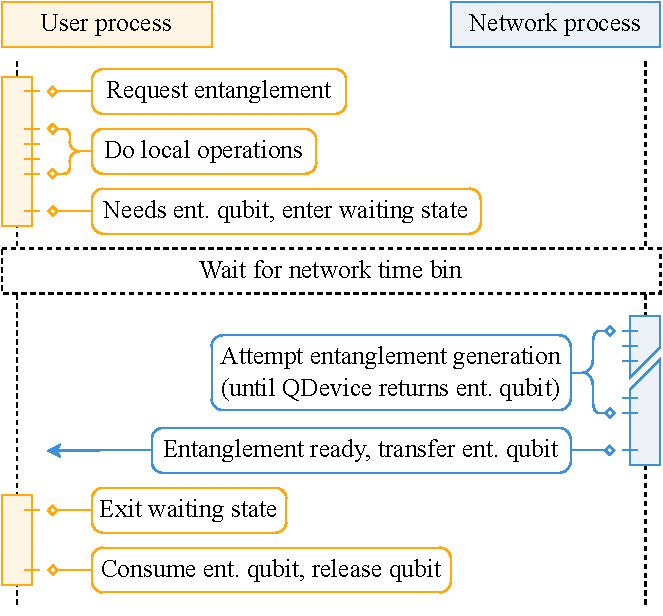
\includegraphics[width=0.6\linewidth]{figures/process-flow.pdf}
    \caption{
        Flow of execution between a user process requesting entanglement and the network process
        responsible for generating entanglement. The user process starts by issuing an asynchronous
        entanglement request. Once issued, it is free to continue with other local operations or
        classical processing. Once it reaches a point in its execution where entanglement is
        required the process enters the waiting state. The network process is then scheduled once
        the appropriate time bin starts, as determined by the network schedule. Once it is running,
        the network process attempts entanglement generation until entanglement success (or until a
        set timeout). The entangled qubit is then transferred to the user process. This unblocks the
        process which consumes the entanglement and releases the qubit.
    }
    \label{fig:process-flow}
\end{figure}

\paragraph{Process flow}

\Cref{fig:process-flow} illustrates the typical control flow between a user process and the network
process. User processes are free to execute any non-networked instructions independently of the
network process and other user processes. Once the application reaches a point in its execution
where an entangled qubit is required, the process enters the waiting state and is flagged as waiting
for entanglement. When the network process is scheduled, it issues network instructions and
generates entanglement as requested by the user process. Once an entangled pair is generated by the
network process, the qubit is handed over to the waiting user process. When all the entangled pairs
that the user process was waiting for are delivered, the user process becomes ready and can start
running again.

\subsection{Process Scheduling}

As previously mentioned, we focus our attention on the quantum blocks of an application, and thus we
only discuss the scheduling of \acrshort{qnodeos} processes. At present, the \acrshort{qnodeos}
scheduler does not give any guarantees on when a process is scheduled --- for that, one would need
to define concrete real-time constraints to feed to the scheduler. Instead, the current version of
\acrshort{qnodeos} implements a best-effort scheduler, which selects processes on the basis of their
priority, and does not allow preemption. The scheduling algorithm is represented in the flowchart in
\cref{fig:scheduler}.

\begin{figure}[t]
    \centering
    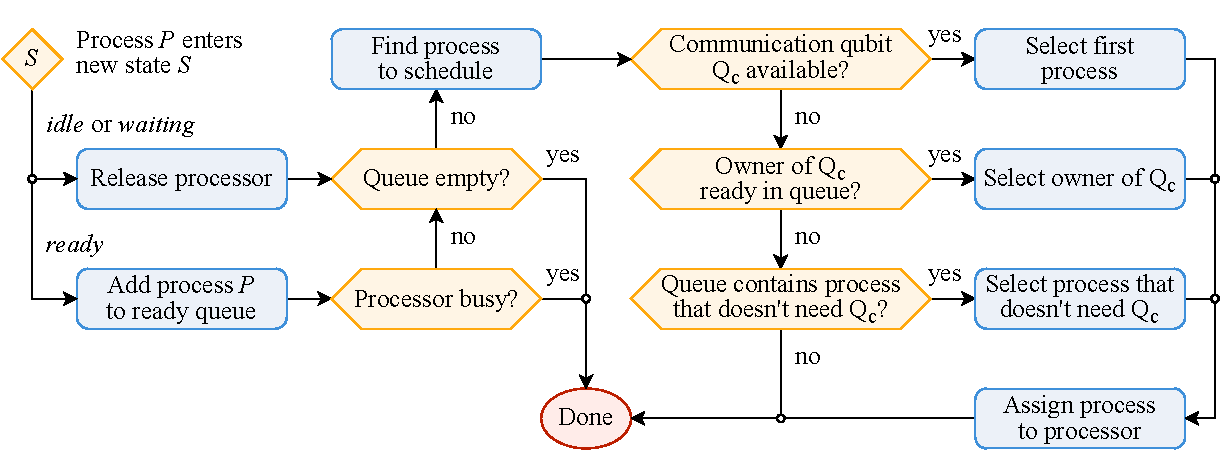
\includegraphics[width=\linewidth]{figures/scheduler.pdf}
    \caption[]{
        Schematic representation of the scheduling algorithm employed by \acrshort{qnodeos}. The
        scheduler is activated when a process $P$ transitions to a new state $S$. If $S$ is
        \emph{idle} or \emph{waiting}, the process has (temporarily) terminated its execution, and
        thus relinquished the processor, in which case the scheduler can proceed. If $S$ is
        \emph{ready}, the process is added to the prioritized ready queue, and if the processor is
        not already busy, the scheduler can proceed again. When the ready queue is not empty, the
        scheduler looks for the next scheduling candidate as follows:
        \begin{inlinelist}
            \item if the communication qubit is available, the scheduler simply selects the
                  highest-priority process in the ready queue;
            \item otherwise, if the process owning the communication qubit is waiting in the ready
                  queue, the scheduler selects this process as the scheduling candidate;
            \item as a last resort, the scheduler searches the ready queue for a process that does
                  not need the communication qubit.
        \end{inlinelist}
        At the moment, the scheduling algorithm is tuned to \acrshort{nv} center-based quantum
        platforms, where the communication qubit plays a rather central role in both entanglement
        generation and local quantum computation.
    }
    \label{fig:scheduler}
\end{figure}

\paragraph{Priority scheduling}

\acrshort{qnodeos} schedules ready processes using a \emph{priority-based} algorithm. In particular,
the network process is assigned the highest priority, and is given precedence whenever the network
schedule activates it~\cite{skrzypczyk_2021_arch}. Prioritizing entanglement generation over local
operations is key for a node to be able to fulfill its networking duty, and to avoid peer nodes to
waste their resources.

\paragraph{No preemption}

To avoid context switching overhead, potentially leading to degraded fidelity, the
\acrshort{qnodeos} scheduler is \emph{cooperative}. That is, once a process is scheduled, it gets to
run until it either completes all of its instructions or it blocks waiting for entanglement.
Allowing process preemption would need a definition of critical section and could potentially impact
the quality of the affected qubit states.

\subsection{QNodeOS Architecture}

We refer again to \cref{fig:quantum-node}, which illustrates the internals of \acrshort{qnodeos},
and outlines the interactions with the rest of the components of a quantum network node. At its top,
\acrshort{qnodeos} implements an \emph{end-node \acrshort{api} handler} to process requests from the
host. Internally, \acrshort{qnodeos} features a \emph{quantum network stack}, a \emph{process
manager}, a \emph{process scheduler}, a \emph{quantum memory management unit} (\acrshort{qmmu}), and
an \emph{instruction processor}. Actual quantum instructions are offloaded to the underlying quantum
device (\acrshort{qdevice}) through the \emph{\acrshort{qdevice} driver}.

We note that \acrshort{qnodeos} itself is an entirely classical system that interacts with the
quantum hardware (the \acrshort{qdevice}). At the moment, our implementation of \acrshort{qnodeos}
is fully software, including the instruction processor. In general, the system may be implemented
entirely in software running on a classical \acrshort{cpu}, or parts of its functionality may be
implemented in classical hardware (e.g.~\acrshort{fpga} or \acrshort{asic}).

\paragraph{End-node API}

Each user application is registered on \acrshort{qnodeos} by the host through the end-node
\acrshort{api}. Using the same \acrshort{api}, the host can then send quantum code blocks and
receive their results (like measurement outcomes and entanglement generation information). Upon
registration of an application, \acrshort{qnodeos} allocates a new user process. Upon reception of a
quantum code block, the related user process is activated and made eligible for scheduling.

\paragraph{Process manager, scheduler, processor}

The \acrshort{qnodeos} process manager keeps track of existing user and kernel processes and their
execution context. Upon activation, processes are added to a scheduling queue. When selected by the
scheduler, a process is assigned to the \acrshort{qnodeos} processor, which
%
\begin{inlinelist}
    \item executes classical control-flow instructions directly,
    \item offloads local quantum computation to the \acrshort{qdevice}, and
    \item registers entanglement requests with the quantum network stack.
\end{inlinelist}

\paragraph{Quantum network stack}

The role of the quantum network stack in \acrshort{qnodeos} is to abstract the unreliable
entanglement attempts that the \acrshort{qdevice} offers into a robust, multi-node network service.
The network stack can handle entanglement generation requests which specify a number of parameters
--- including source and destination, desired fidelity, and number of entangled pairs --- and
returns the entangled pair(s) described by an identifier and the generated Bell state. The quantum
network stack owns the network process, whose activation is dictated by a network-wide entanglement
schedule. The quantum network stack in \acrshort{qnodeos} is based on the model outlined by
\textcite{dahlberg_2019_egp}, and features a \emph{link layer protocol} --- presented in the same
work, and recently evaluated on hardware~\cite{pompili_2022_experimental} (\cref{chp:netstack}) ---
and a \emph{network layer protocol} --- as designed by \textcite{kozlowski_2020_qnp}.

\paragraph{Quantum memory management unit}

\acrshort{qnodeos}'s \acrshort{qmmu} implements basic memory management functionality: \emph{virtual
address spaces} and \emph{qubit ownership transfer}. A virtual quantum memory address space is akin
to a classical virtual address space, but it isolates the qubit address spaces of \acrshort{qnodeos}
processes. Ownership transfer is an indirect type of \acrfull{ipc} mechanism for passing quantum
data between processes. Since quantum states cannot be copied due to the no-cloning theorem, this is
the only valid \acrshort{ipc} for passing quantum data between address spaces. Ownership transfer is
only logical --- only the data's owner is updated --- rather than it being a physical move of
quantum data in the memory. This way we can avoid issuing a \acrshort{qdevice} instruction which
would cause degradation in fidelity due to hardware imperfections and additional processing time.
The current \acrshort{qmmu} is rather simple due to the fact that our current quantum nodes have
only have a few qubits each. Features like decoherence tracking and topology-based allocation can be
part of a later version of the \acrshort{qmmu}.

\section{Discussion}

We have discussed general design considerations for an \acrshort{os} for quantum network nodes, and
identified the fundamental components of such an \acrshort{os}. We have also presented a reference
architecture that abides by these requirements. Whilst our architecture is a proof of concept, and
is not meant to deliver optimal performance, we implement it and test it to run simple quantum
networking applications. We will proceed to experimentally demonstrate the capabilities of
\acrshort{qnodeos} in \cref{chp:netstack,chp:qnodeos}.

\begin{xstretch}
\printbibliography[heading=subbibintoc,title={References},notcategory=noprint]
\end{xstretch}
